
\chapter{Implementácia}

V kapitole budú opísané podrobné počty dát v daných kategóriách zo zdrojov, ktoré boli uvedené v návrhu (viď. \ref{sec:databaza})
    na ktorých prebieha trénovanie, opíše implementáciu tried, ktoré zabezpečujú načítavanie týchto dát a možnosti ich načítania.
Následne tu budú spomenuté triedy, ktoré zabezpečujú predspracovanie obrazu.
Kapitola ďalej priblíži typy implementovaných modelov, infomácie, ktoré sa po trénováni ukladajú, parametre trénovania a spôsob hodnotenia presnosti modelov.



\section{Trénovacie dáta}
\label{sec:trenovaciedata}

\subsection{Zber dát}
Pre trénovanie modelov boli použité obrázky zo zdrojov spomenutých v kapitole \ref{sec:databaza}.
Tabuľka nižšie uvádza podrobné počty obrázkov z daných zdrojov ktoré boli použité pre určenie typu zbrane v 2 kategóriách.

\begin{table}[H]
  \centering
  \label{my-label}
  \begin{tabular}{|l|c|c|}
    \hline
    Zdroj               & \multicolumn{1}{l|}{Počet krátkych zbraní} & \multicolumn{1}{l|}{Počet dlhých zbraní} \\ \hline
    IMFDB               & 647                                        & 670                                      \\ \hline
    ImageNet            & 730                                        & 94                                       \\ \hline
    Google vyhľadávanie & 0                                          & 86                                       \\ \hline \hline
    SPOLU               & 1377                                       & 850                                      \\ \hline
  \end{tabular}
  \caption{Podrobné počty trénovacích dát.}
\end{table}

Vo všeobecnosti je jednoduchšie nájsť obrázky ktoré obsahujú krátke zbrane (pištole) ako dlhé zbrane.
Databáza ImageNet obsahovala vyše 3000 odkazov na obrázky, avšak veľká časť z nich bola chybná alebo daný súbor už neexistoval.

Ako bolo spomínané v \ref{subsec:generovanie3d}, obrázky ktoré boli použité na trénovanie modelov pre určenie náklonu zbrane bolo potrebné
    vygenerovať pomocou 3D modelov.
Pre toto generovanie bolo použitých desať pozadí scény a päť 3D modelov z toho tri modely boli dlhé zbrane a dve modely krátkych zbraní.

\begin{figure}[H]
    \centering
    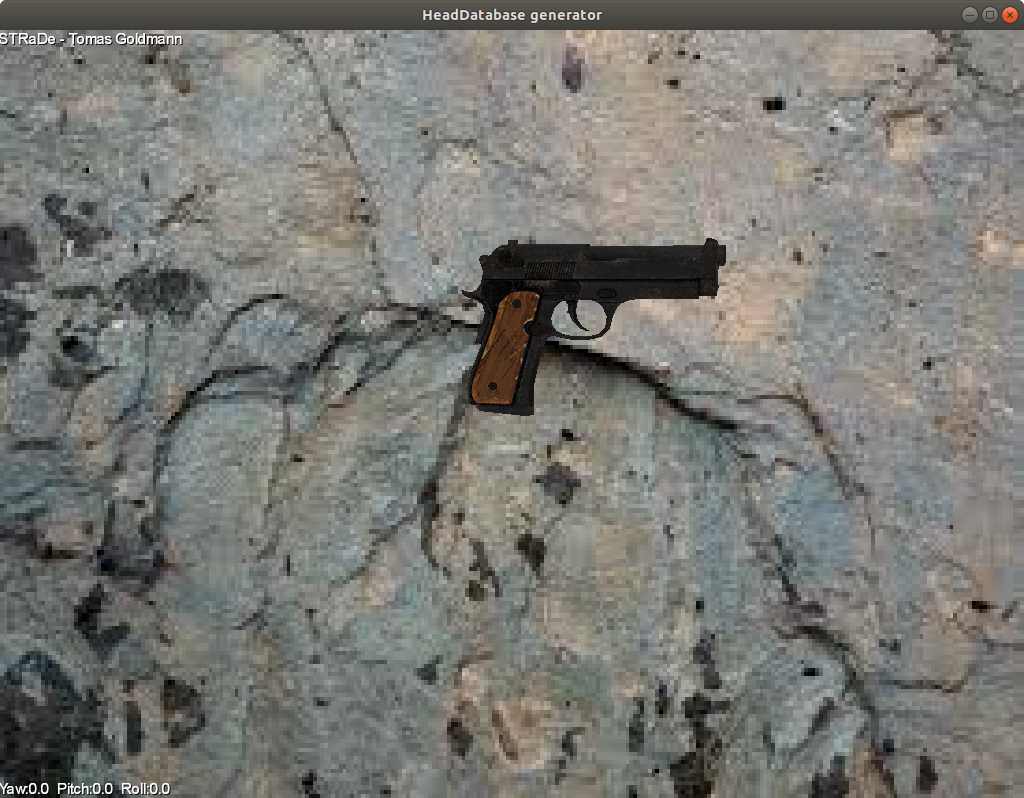
\includegraphics[width=0.7\textwidth]{generator3d}
    \caption{Program pre generovanie obrázkov z 3D modelov.}
    \label{pic:generator3d}
\end{figure}

Niektoré použité modely mali nastavený zlý bod otáčania a taktiež boli veľmi malé.
Preto, ako je vidieť na obrázku \ref{pic:generator3d}, museli byť výsledne obrázky ešte orezané aby sa vnich nachádzala iba zbran bez nepotrebného okolia.

\begin{figure}[H]
    \centering
    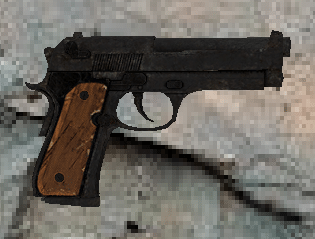
\includegraphics[width=0.5\textwidth]{croped_weapon}
    \caption{Výsledný vygenerovaný obrázok po orezaní okolia.}
    \label{pic:generator3d}
\end{figure}

Tabuľka nižsie uvádza presné počty vygenerovaných obrázkov.

\begin{table}[H]
    \centering
    \label{my-label}
    \begin{tabular}{|l|c|}
        \hline
        Typ osi otáčania & \multicolumn{1}{l|}{Počet obrázkov} \\ \hline
        pitch            & 1480                                \\ \hline
        roll             & 4450                                \\ \hline
        yaw              & 4600                                \\ \hline
        \end{tabular}
    \caption{Podrobné počty trénovacích dát.}
\end{table}

Pre os otáčania pitch boli vybrané obrázky z datasetu určeného pre klasifikáciu typu zbrane.
Pre zvyšné 2 osi boli obrázky generované, počty sa líša kvôli niektorým chybným obrázkom ktoré museli byť vymazané.

\subsection{Načítavanie dát}
\label{subsec:nacitaniedat}
Pre načítavanie dát je implementovaná trieda \textit{DataLoader} v scripte \textit{loader.py}.
Trieda obsahuje niekoľko funkcií pre načítanie týchto dát, tieto funkcie vrátia pole načitaných obrázkov, pole indexov označení [eng. labels] obrázkov a
    štruktúru typu dictionary ktorá obsahuje index a názov označenia, napr. \{0: ``kratka zbran'', 1: ``dlha zbran''\}.

Prvá z funkcií načitáva dáta z priečinka kde označenie obrázkov, či je to krátka alebo dlhá zbraň, je zabezpečené podľa názvou podpriečinkou.
Pre obrázky o náklne zbrane sa označenie osi berie takisto z názvu podpriečinka, avšak presné označenie o koľko stupňov je model v obrázku otočený
    je získaný z názvu obrázka ktorý musí spĺnať presný formát: \textit{p0.0\_y0.0\_r0.0-typzbrane.jpg}.
Kde \textit{p0.0} označuje hodnotu náklonu v osi pitch, \textit{y0.0} hodnotu náklonu v osi yaw, \textit{r0.0} v osi roll a \textit{typzbrane} môže byť
    akýkoľvek reťazec.
Formát vstupných obrázkov môže byť \textit{.jpg} alebo \textit{.jpeg}.

Správnu hierarchiu priečinkou je vidieť na obrázoku \ref{pic:folderhierarchy}

\begin{figure}[H]
    \centering
    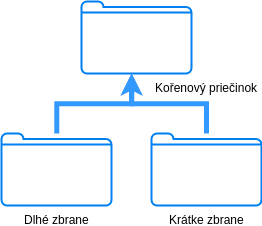
\includegraphics[width=0.32\textwidth]{class_hierarchy}
    \qquad
    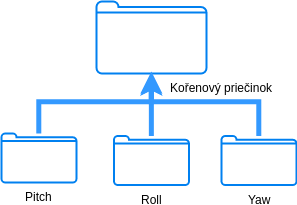
\includegraphics[width=0.4\textwidth]{angle_hierarchy}
    \caption{Hierarchia priečinkou pre správne označenie vstupných obrázkov.}
    \label{pic:folderhierarchy}
\end{figure}

Druhá z funkcií umožňuje načítať zoznam obrázkov z textového súboru, kde sa na každom riadku nachádza práve jedna cesta k požadovanému obrázku.
Spôspob označovania obrázkov je rovnaký ako v prvom prípade, preto je taktiež potrebné dodržat správnu hierachiu priečinkou.

\subsection{Predspracovanie dát}
\label{subsec:predspracovaniedat}
Pre predspracovanie obrazu sú implementované 2 triedy \textit{Preprocessor} a \textit{Preprocessing} v scripte \textit{preprocessing.py}.
Trieda \textit{Preprocessor} obsahuje list do ktorého je možné pridávať funckíe ktoré sú implementované v triede \textit{Preprocessing}.
Po zavolaní funkcie \textit{apply(input\_data)} z triedy \textit{Preprocessor}, sa tieto
    funkcie v poradí v akom boli pridané do listu zavolajú a prebehne predspracovanie vstupných dát.
Každá z možností predspracovanie obrazu ktorá bola uvedená v \ref{sec:preprocessing}, je implementovaná v triede \textit{Preprocessing} pomocou
    knižnice scikit-image.

Pre augmentáciu dát určených na klasfikáciu typu zbrane je použitá trieda \textit{ImageDataGenerator} z knižnice Keras.
Parametre tohto generátora sú nastavená na: horizonálne a vertikálne preklopenia obrázka, posun obrázka až o 15\% jeho dĺžky alebo šírky,
    rotácia o náhodný uhol v rozsahu 0 až 180 stupňov a doplnenie čiernych pixelov pomocou nastavenia ``nearest''.

Pre augmentáciu dát pre určenie náklonu zbrane je implementovaná samostatná trieda \textit{AngleGenerator}, ktorá zabezpečuje správne dogenerovanie
    vstupných dát pomocou horizontálneho alebo vertikálneho preklopenia obrázka a správneho výpočtu uhlu natočenia (viď. \ref{subsec:augmentacia}).



\section{Modely}
\label{sec:modely}
Všetky modely pre trénovanie su implementované v scripte \textit{models.py}.
Existuje jedna hlavná trieda \textit{class Model}, ktorá obsahuje všetky základne atributy potrebné pre modely, ako npr.
    meno modelu, vstupný rozmer dát, zvolený algoritmus trénovania a štruktúru typu dictionary ktorá obsahuje indexi a názvi označení obrázkov.

Každý model následne dedí z tejto hlavnej triedy a implementuje v sebe 2 funkcie \textit{build} ktorá zabezpečuje vytvorenie modelu a
    funkciu \textit{train} ktorá sa volá pri spustení trénovania daného modelu.

\begin{figure}[H]
    \centering
    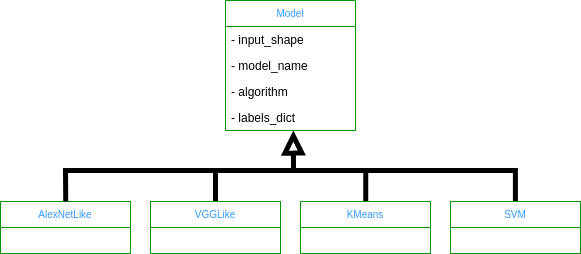
\includegraphics[width=0.8\textwidth]{inheritance}
    \caption{Hierarchia dedenia tried modelov.}
    \label{pic:inheritance}
\end{figure}

Konvolučné neurónové siete su implementované pomocou triedy \textit{Sequencia} z knižnice Keras.
Pre klasifikátor K-Nearest-Neighbor je použitá trieda \textit{KNeighborsClassifier} a trieda \textit{SVC} pre klasifikátor SVM z knižnice scikit-learn.
%Pre klasifikátor K-Nearest-Neighbor je použitá trieda \textit{KNeighborsClassifier} s počtom 1 a 5 najbližších susedov, a trieda \textit{SVC} pre klasifikátor SVM
%    so základnymi nastavenia trénovania z knižnice scikit-learn.

\subsection{Ukladanie a načitanie modelu}
\label{subsec:ukladaniemodelu}
Pre ukladanie natrénovaných modelov je implemtovaná funkcia \textit{save\_model()} v triede \textit{DataSaver} v scripte \textit{loader.py}.
Pri ukladaní modelu sa ukladá model v binárnej forme, ukladá sa konfiguračný súbor \textit{settings.json} ktorý obsahuje informácie ako veľkosť
    vstupných dát, použité funkcie na predspracovanie dát, meno modelu, typ algoritmu učenia, zoznam indexov označenia dát a dalšie informácie
    špecifické pre daný typ modelu.
Uložením konvolučnéj neurónovej siete sa ukladá graf priebehu trénovanie.

Naopak pre načitanie modelov je implementovaná funkcia \textit{load\_model\_data()} v triede \textit{DataLoader} v scripte \textit{loader.py},
    ktorá načíta binárnu podobu modelu a všetky informácie z konfiguračného súboru \textit{settings.json}.



\section{Trénovanie modelov}
\label{sec:trenovanie}
Pre trénovanie modelov sú v rámci implementácie použité všetky triedy ktoré boli podrobne opísane vyššie.
Proces trénovania prebieha v niekoľkých krokoch.
\begin{enumerate}
    \item[$\bullet$] Načítanie vstupných dát.
    \item[$\bullet$] Predspracovanie načitaných dát.
    \item[$\bullet$] Rozdelenie predspracovaných dát na trénovacie, validačné a testovanie v pomere 70\%:15\%:15\% pre konvolučné neurónové siete.
    A v pomere 70\%:30\% na trénovacie a testovanie pre K-means a SVM klasifikátor.
    \item[$\bullet$] Vytvorenie modelu.
    \item[$\bullet$] Spustenie trénovania vytvoreného modelu.
    \item[$\bullet$] Uloženie natrénovaného modelu a konfiguračného súboru.
    \item[$\bullet$] Testovanie presnosti modelu pomocou testovacích dát.
\end{enumerate}

Pre uľahčenie trénovania je implementovaný script \textit{train.py} ktorý požaduje niekoľko argumentov na vstupe.
Zoznam vstupných argumentov a ich význam, argumenty v hranatých zátvorkách sú voliteľné:
\begin{enumerate}
  \item[$\bullet$] \textbf{--model} cesta k priečinku do ktorého bude natrénovaný model uložený.
  \item[$\bullet$] \textbf{--dataset} cesta k priečinku z ktorého budu načítane vstupné dáta.
  \item[$\bullet$] \textbf{--alg} voľba modelu ktorý bude trénovaný, tento argument má niekoľko možností.
  Možnosť ``cnnc'' pre trénovanie konvolučnej neurónovej siete určenej na klasifikáciu zbrane,
  ``cnna'' pre trénovanie konvolucnej neurónovej siete pre určenie náklonu zbrane a
  ``svm'' alebo ``kmeans'' pre trénovanie SVM alebo K-nearest-neighbor klasifikátora na určenie typu zbrane.
  \item[$\bullet$] \textbf{[--ep]} pri konvolučných neurónových sieťach určuje počet epóch, pri jeho nezadaní je použitá
  základné hodnota 45.
  \item[$\bullet$] \textbf{[--bs]} určuje veľkosť batch-size pri trénovaní konvolučných neurónových sietí, jeho
  základná hodnota je 16.
  \item[$\bullet$] \textbf{[--rt]} je argument ktorý je potrebné zadať pri trénovani sietí na určenie náklonu zbrane,
  jeho hodnota určuje uhol náklonu na ktorý sa sieť bude učiť, možné hodnoty argumentu sú: ``yaw'', ``roll'', ``pitch''.
\end{enumerate}

\subsection{Hodnotenie presnosti modelov}
\label{subsec:hodnoteniepresnosti}
Pre celkové hodnotenie presnosti modelov bola implementovaná funkcia \textit{evaluate\_model} v scripte \textit{evaluation.py}.
Ktorá hodnotí presnosť sieťe podľa nižšie spomínaných metrík.

V prípade určenia typu zbrane sa používa tzv. chybová alebo tiež kontigenčná matica.
Kde každý stĺpec v matici predstavuje klasifikované triedy a jednotlivé riadky predstavujú správne triedy.
Tabuľka \ref{tab:chybovamatica} zobrazuje túto maticu.
Hodnota TP označuje počet správne klasifikovaných obrázkov triedy true, hodnota FP označuje počet nesprávne klasfikovaných obrázkov triedy true.
Hodnota TN označuje poćet správne klasifikovaných obrázkov triedy false, hodnota FN označuje počet nesprávne klasifikovaných obrazkov triedy false \cite{odkaz:ChybovaMatica}.
\begin{table}[H]
    \centering
    \label{tab:chybovamatica}
        \begin{tabular}{lllc}
                                                                &                                   & \multicolumn{2}{c}{Klasifikované hodnoty}                                           \\ \cline{3-4} 
                                                                & \multicolumn{1}{l|}{}             & \multicolumn{1}{c|}{Trieda false}        & \multicolumn{1}{c|}{Trieda true}         \\ \cline{2-4} 
        \multicolumn{1}{c|}{\multirow{2}{*}{Správne hodnoty}} & \multicolumn{1}{c|}{Trieda false} & \multicolumn{1}{l|}{TN (True Negative)}  & \multicolumn{1}{c|}{FP (False Positive)} \\ \cline{2-4} 
        \multicolumn{1}{c|}{}                                 & \multicolumn{1}{c|}{Trieda true}  & \multicolumn{1}{l|}{FN (False Negative)} & \multicolumn{1}{c|}{TP (True Positive)}  \\ \cline{2-4} 
    \end{tabular}
    \caption{Chybová matica}
\end{table}
Pre prípad tejto práce si môžeme preniesť triedu true na triedu krátke zbrane a triedu false na triedu dlhé zbrane.
Ako hodnotenie presnosti bude použitá metrika úspešnosť [eng. Accuracy].

Úspešnosť - táto hodnota určuje ako často klasfikátor správne klasifikoval daný obrázok, počíta sa ako:
\begin{equation}
    Accuracy = \frac{TP + TN}{TP + TN + FP + FN}
\end{equation}
Táto metrika je použitá aj počas trénovania sietí na predbežné určenie presnosti a taktiež pri koncovom testovaní modelu.

Avšak v prípade siete ktorá určuje náklon zbrane je potrebné túto metriku trošku pozmeniť.
Ako je opísane v \ref{subsec:odchylkachyby}, v scripte \textit{base.py} je implementovaná funkcia \textit{angle\_error} ktorá ráta priemerny rozdiel medzi
    skutočnymi a predpovedanými uhlami siete.
Táto funkcia je použita ako metrika počas trénovania siete, pri koncovom testovaní presnosti siete je nastavená prahová hodnota uhla podľa ktorej sa určuje,
    či daná predpoveď siete bola správna alebo nie.
Správne určenie je vypočítane ako rozdiel medzi skutočným uhlom a predpovedaným uhol pomocou siete, ak je rozdiel menší ako prehová hodnota, tak predikcia
    sa považuje za správnu.
Toto koncové testovanie siete už využíva metriku presnosti podľa chybovej matice.



\section{Zhrnutie kapitoly}

Kapitola v úvode uvádza presné počty dát, podľa zdrojov, ktoré sú použité pre tŕenovanie modelov.
Vysveťluje postup generovania obrázkov z 3D modelov.
Ďalej sa venuje možnostiam načítavania dát zo súbora alebo priečinkov pri doržaní potrebnej hierarchie priečinkov a názvu súborov.
Približuje triedy, ktoré implementujú predspracovanie vstupných dát, tvorbu modelov, uvádza informácie ktoré sú uložené
    pri ukladaní modelov a spôsob ich načítania.
Nasleduje celý postup trénovania modelov, opis scriptu, ktorý toto trénovanie uľahčuje a vysveťluje metriky, podľa ktorých sa hodnotí presnosť modelov.
